\begin{figure}[ht] 
 	\centering 
 	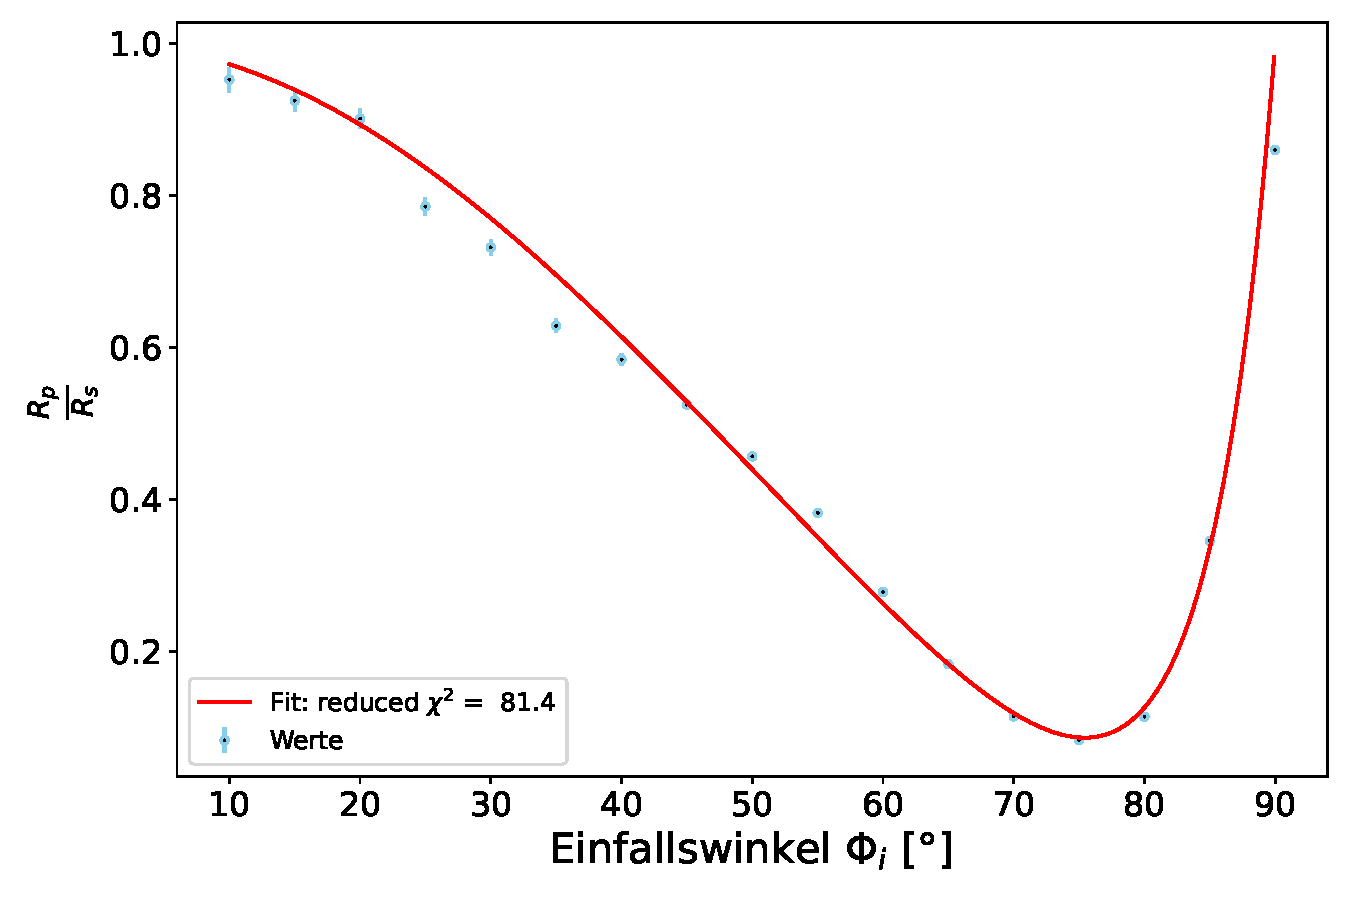
\includegraphics[width= 0.65 \textwidth]{Fits/Rp_Rs_Cu_Fit.pdf} 
	\caption{Rp Rs Cu, Fit} 
 	\label{fig:Rp Rs Cu, Fit} 
\end{figure}
 
\begin{table}[ht] 
	\centering 
	\caption{Rp Rs Cu, Fit Parameter Tabelle} 
	\label{tab: Rp Rs Cu, Fit Parameter Tabelle}
	\begin{tabular}{|l|c|}
		\hline
		Parameter Name	&	Wert \\ \hline
		n	&	 3.2437 $\pm$  0.135\\ \hline
		kappa	&	-1.95106 $\pm$  0.05857\\ \hline
	\end{tabular} 
\end{table}
 
\begin{table}[ht] 
	\centering 
	\caption{Rp Rs Cu, Messwerte Tabelle} 
	\label{tab: Rp Rs Cu, Messwerte Tabelle}
	\begin{tabular}{|c|c|}
		\hline
		Einfallswinkel $\Phi_i$ [°] 	&	 $\frac{R_p}{R_s}$\\ \hline
		90.0 $\pm$ 0.2 	&	 0.8600 $\pm$ 0.0044 \\ \hline
		85.0 $\pm$ 0.2 	&	 0.3455 $\pm$ 0.0024 \\ \hline
		80.0 $\pm$ 0.2 	&	 0.1137 $\pm$ 0.0027 \\ \hline
		75.0 $\pm$ 0.2 	&	 0.0832 $\pm$ 0.0029 \\ \hline
		70.0 $\pm$ 0.2 	&	 0.1143 $\pm$ 0.0035 \\ \hline
		65.0 $\pm$ 0.2 	&	 0.1829 $\pm$ 0.0008 \\ \hline
		60.0 $\pm$ 0.2 	&	 0.2782 $\pm$ 0.0043 \\ \hline
		55.0 $\pm$ 0.2 	&	 0.3821 $\pm$ 0.0049 \\ \hline
		50.0 $\pm$ 0.2 	&	 0.4566 $\pm$ 0.0057 \\ \hline
		45.0 $\pm$ 0.2 	&	 0.5247 $\pm$ 0.0064 \\ \hline
		40.0 $\pm$ 0.2 	&	 0.5841 $\pm$ 0.0075 \\ \hline
		35.0 $\pm$ 0.2 	&	 0.6286 $\pm$ 0.0092 \\ \hline
		30.0 $\pm$ 0.2 	&	 0.7318 $\pm$ 0.0108 \\ \hline
		25.0 $\pm$ 0.2 	&	 0.7855 $\pm$ 0.0115 \\ \hline
		20.0 $\pm$ 0.2 	&	 0.9013 $\pm$ 0.0133 \\ \hline
		15.0 $\pm$ 0.2 	&	 0.9247 $\pm$ 0.0146 \\ \hline
		10.0 $\pm$ 0.2 	&	 0.9526 $\pm$ 0.0164 \\ \hline
	\end{tabular} 
\end{table}
 
